% Exercise Template
%A LaTeX template for typesetting exercise in Persian (with cover page).
%By: Reza Adinepour

\documentclass[12pt]{exam}

\usepackage{setspace}
\usepackage{listings}
\usepackage{graphicx,subfigure,wrapfig}
\usepackage{multirow}
\usepackage{matlab-prettifier}
\usepackage{amsmath}
\usepackage{multicol}


\usepackage[margin=20mm]{geometry}
\usepackage{xepersian}
\settextfont{XB Niloofar}

\newcommand{\class}{آزمایشگاه DSP}
\newcommand{\term}{نیم‌سال دوم ۰۱-۰۲}
\newcommand{\college}{دانشکده مهندسی برق}
\newcommand{\prof}{استاد: دکتر مقیمی}

\singlespacing
\parindent 0ex

\begin{document}


% -------------------------------------------------------
%  Thesis Information
% -------------------------------------------------------

\newcommand{\ThesisType}
{سمینار}  % پایان‌نامه / رساله
\newcommand{\ThesisDegree}
{کارشناسی ارشد گرایش معماری کامپیوتر}  % کارشناسی / کارشناسی ارشد / دکتری
\newcommand{\ThesisMajor}
{مهندسی برق}  % مهندسی کامپیوتر
\newcommand{\ThesisTitle}
{موضوع آزمایش}
\newcommand{\ThesisAuthor}
{رضا آدینه پور-9814303\\علی‌رضا قربانی-9823263}
\newcommand{\ThesisSupervisor}
{جناب آقای دکتر رضا خرقانیان}
\newcommand{\ThesisDate}
{اردی‌بهشت 1402}
\newcommand{\ThesisDepartment}
{دانشکده مهندسی برق}
\newcommand{\ThesisUniversity}
{دانشگاه صنعتی شاهرود}

% -------------------------------------------------------
%  English Information
% -------------------------------------------------------

\newcommand{\EnglishThesisTitle}{A Standard Template for Course Exercise}


\pagestyle{empty}

\begin{center}


\includegraphics[scale=0.17]{images/logo.png}

\vspace{0.5cm}
\ThesisUniversity \\[-0.3em]
\vspace{0.5cm}
\ThesisDepartment\\

\begin{large}
\vspace{0.5cm}


%\ThesisMajor

\end{large}

\vspace{1.5cm}

{عنوان:}\\[1.2em]
{\LARGE\textbf{\ThesisTitle}}\\ 
\vspace{1cm}
% \begin{latin}
% {\Large\textbf\EnglishThesisTitle}
% \end{latin}

\vspace{2cm}

{نگارش}\\[.5em]
{\large\textbf{\ThesisAuthor}}

\vspace{1.5cm}

{استاد مربوطه}\\[.5em]
{\large\textbf{\ThesisSupervisor}}

\vspace{1cm}



\vspace{2cm}

\ThesisDate

\end{center}

\newpage


% These commands set up the running header on the top of the exam pages
\pagestyle{head}
\firstpageheader{}{}{}
\runningheader{صفحه \thepage\ از \numpages}{}{\class}
\runningheadrule

\vspace{0pt}




\begin{questions}
\pointpoints{نمره}{نمره}

\question
در نرم افزار متلب، با استفاده از تابعی که در تمرین اول نوشتید یک تابع سینوسی با فرکانس نمونه برداری 16 کیلوهرتز، به مدت 2 ثانیه و با فرکانس دقیق 1000 هرتز ایجاد کنید. با هر روشی که می‌توانید در متلب در حوزه فرکانس این سیگنال را برسی و فرکانس آن را استخراج کنید. انتظار می‌رود 1000 هرتز باشد. آیا دقیقا همان مقدار است؟ در صورت تفاوت علت را توضیح دهید. \\

• کد نوشته شده به‌صورت زیر است: \\
\begin{latin}
\begin{lstlisting}[
	frame=single,
	numbers=left,
	style=Matlab-editor %style: % Matlab-editor, Matlab-Pyglike, Matlab-bw
	] 
clear; clc; close all;

% Generate a sinusoidal signal in 0 to 1 sec with:
% signal frequency = 1 kHz
% sampling frequency = 16 kHz

f = 1e3;
fs = 16e3;
T = 10;

% Generate a sinusoidal signal
[y t] = mySin(f, fs, T);

% Compute Fourier transform of the signal
y_fourier = fft(y);
N = length(y);
X_mag = abs(y_fourier(1:N/2+1)); % Magnitude of positive frequency components
frequencies = linspace(0, fs/2, N/2+1); % Frequencies corresponding to positive frequency components

% Plot magnitude of Fourier transform versus frequency
figure(1);
subplot(3, 1, 1);
plot(t, y);
title(['input signal with f = ', num2str(f), 'Hz']);
xlim([0, 0.005]);

subplot(3, 1, 2);
plot(t, abs(fftshift(y_fourier)));
title('fourier transform of input signal');

subplot(3, 1, 3)
plot(frequencies, X_mag);
title('frequency spectrum');
xlabel('Frequency (Hz)');
ylabel('Magnitude');

\end{lstlisting}
\end{latin}

• خروجی برنامه به‌صورت زیر است: 
\begin{figure}[t]
	\centering
	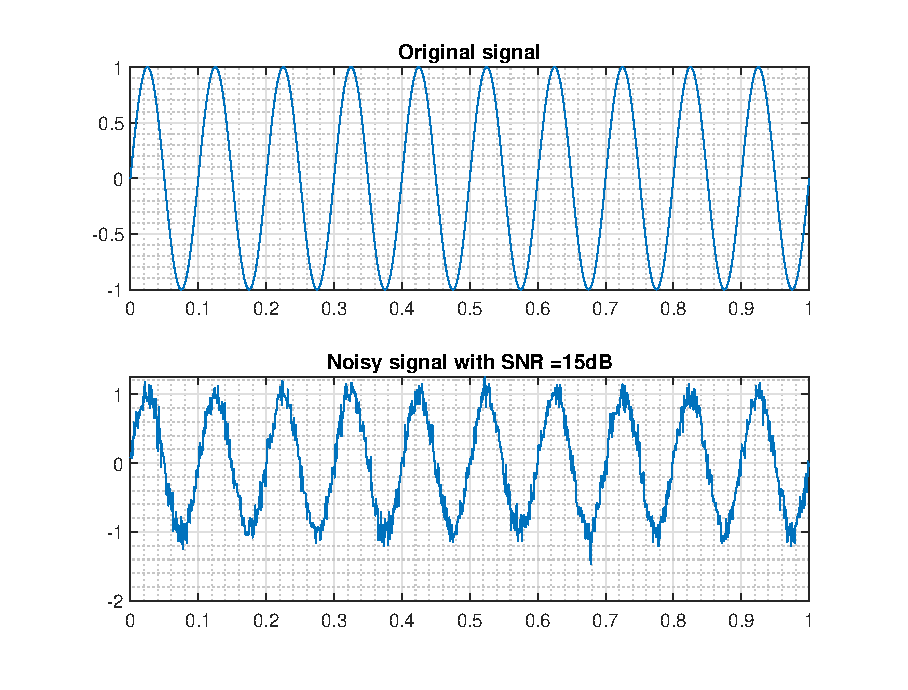
\includegraphics[width=1\textwidth]{images/Result}
	\caption{خروجی برنامه}
\end{figure}

با توجه یه خروجی برنامه مشاهده می‌شود که فرکانس سیگنال دقیقا همان 1 کیلوهرتز بدست آمده است.


\end{questions}
\end{document}

